\chapter{Briefe setzen}
\label{Kapitel_Briefe}
\index{Brief}

Es existieren mehrere Erweiterungspakete, von denen jedes ein Layout und eine Reihe von Befehlen definiert, 
um das Setzen von Briefen zu erleichtern. 
Die Dokumentklasse \verb!letter! ist auf den englischen Sprachraum zugeschnitten und wird in diesem Dokument nicht weiter vertieft. Für Briefe nach deutschem Standard sind die Dokumentklassen \verb!dinbrief!, \verb!g-brief! oder \verb!g-brief2! besser geeignet. 
Eine moderne Alternative ist zudem die KOMA-Klasse \verb!scrlttr2!. 

In diesem Dokument ist der Fokus auf je einem funktionierenden Beispiel mit \verb!g-brief2! und \verb!scrlttr2!. Beide Dokumentklassen definieren eine Reihe selbsterklärender Befehle. 

\section{Briefe mit der Dokumentklasse \texttt{g-brief2}}
\index[cmd]{\texttt{g-brief2}}

Zur Dokumentklasse \verb!g-brief2! existiert vom Autor Michael Lenzen eine gut verständliche Dokumentation~\cite{gbrief_Dokumentation} in deutscher Sprache.  

\lstinputlisting[caption={Ein Beispiel zur Dokumentklasse \texttt{g-brief2}},label=beispielgbrief2, style=customlatex]{Beispiele/Brief_gbrief2/brief_gbrief2.tex}


\begin{figure}[H]
%     \centering
         % Abschneiden mit trim = liks unten rechts oben
         \fbox{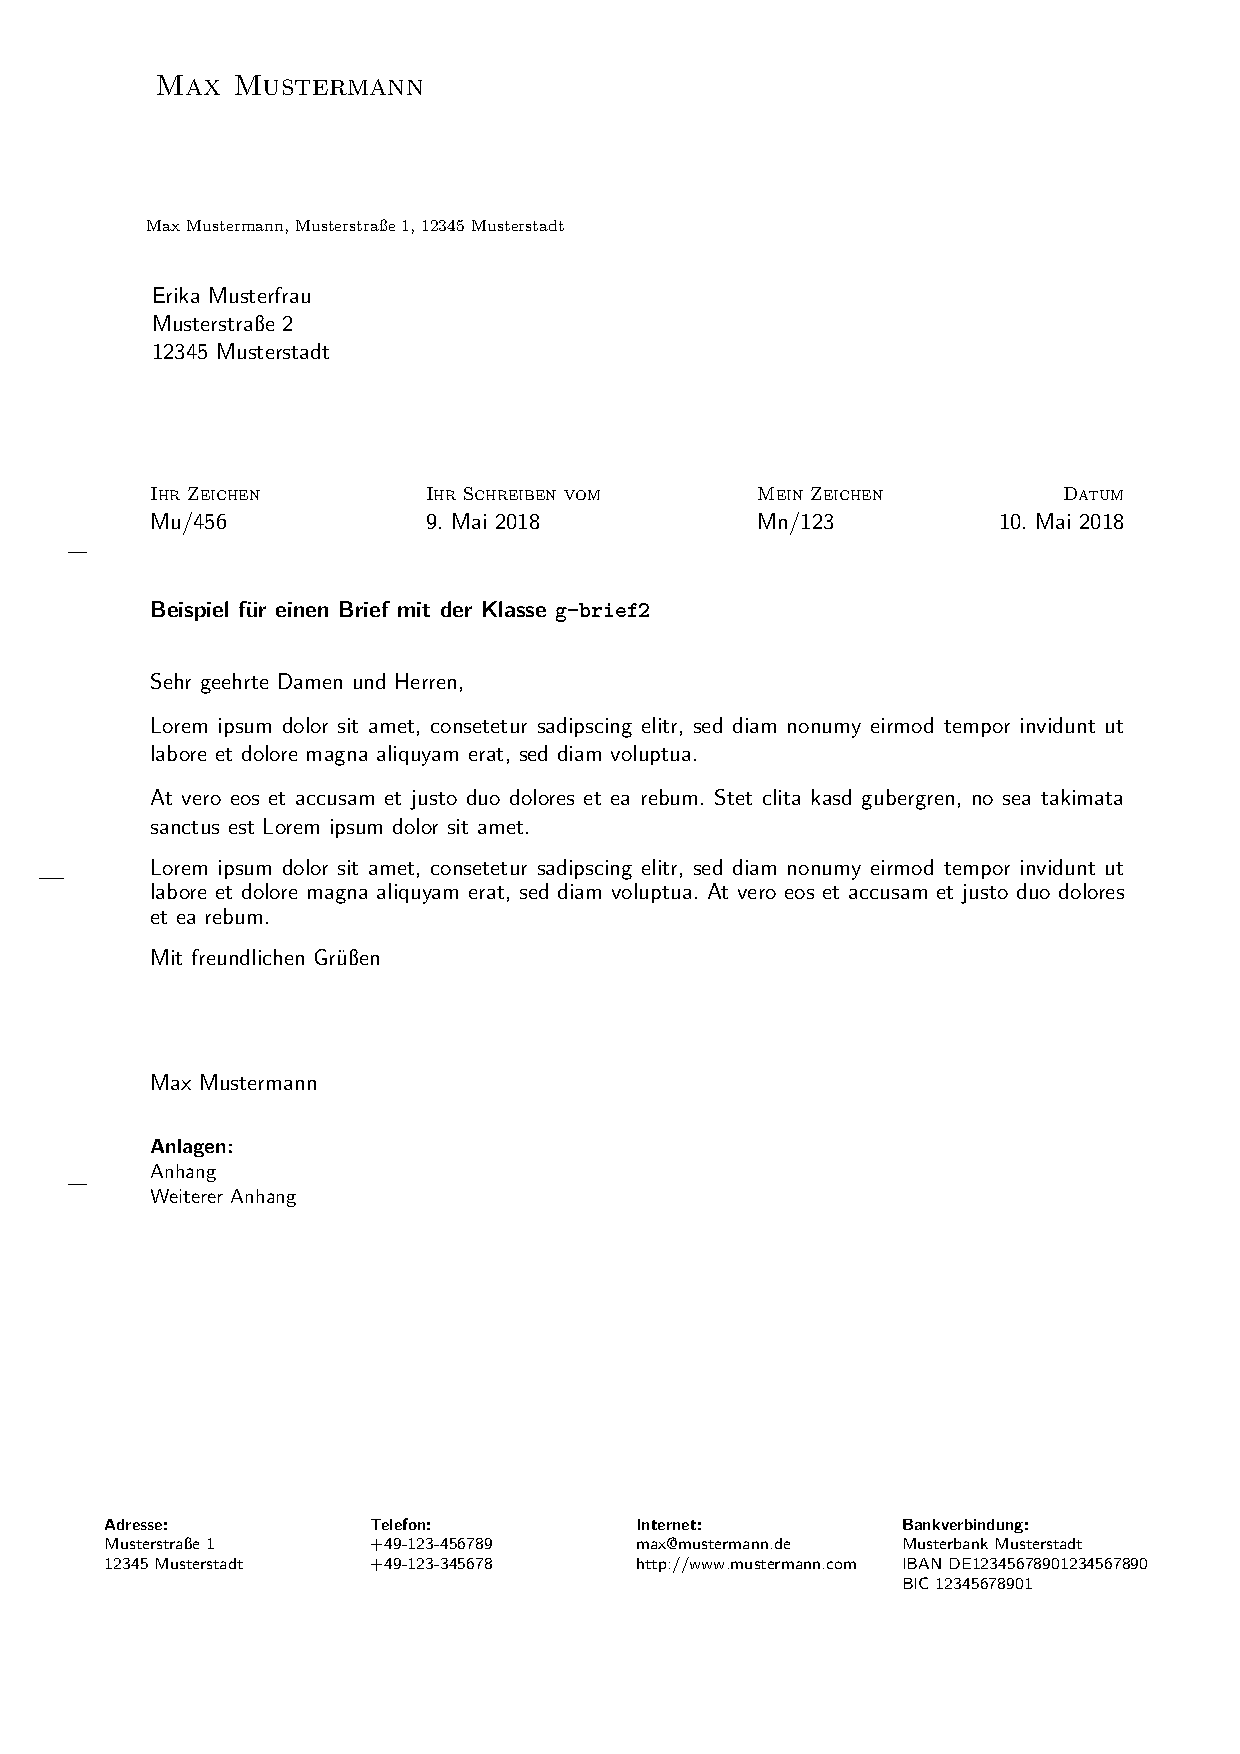
\includegraphics[page=1, width=.98\textwidth]{Beispiele/Brief_gbrief2/brief_gbrief2.pdf}}
    \caption{Resultat von Listing~\ref{beispielgbrief2}}
    \label{fig_gbrief2}
\end{figure}


\section{Briefe mit der Dokumentklasse \texttt{scrlttr2}}
\index[cmd]{\texttt{scrlttr2}}

Eine moderne Alternative zur Dokumentklasse \verb!g-brief2! ist die Klasse \verb!scrlttr2!. Diese ist Teil des \LaTeXe-Erweiterungspakets KOMA-Script. Die Klasse bietet vielfältige Optionen zur Briefgestaltung und ist auch in deutscher Sprache umfangreich dokumentiert~\cite{KOMAScript_Dokumentation}.

\lstinputlisting[caption={Ein Beispiel zur Dokumentklasse \texttt{scrlttr2}},label=beispielscrlttr2, style=customlatex]{Beispiele/Brief_scrlttr2/brief_scrlttr2.tex}


\begin{figure}[H]
%     \centering
         % Abschneiden mit trim = liks unten rechts oben
         \fbox{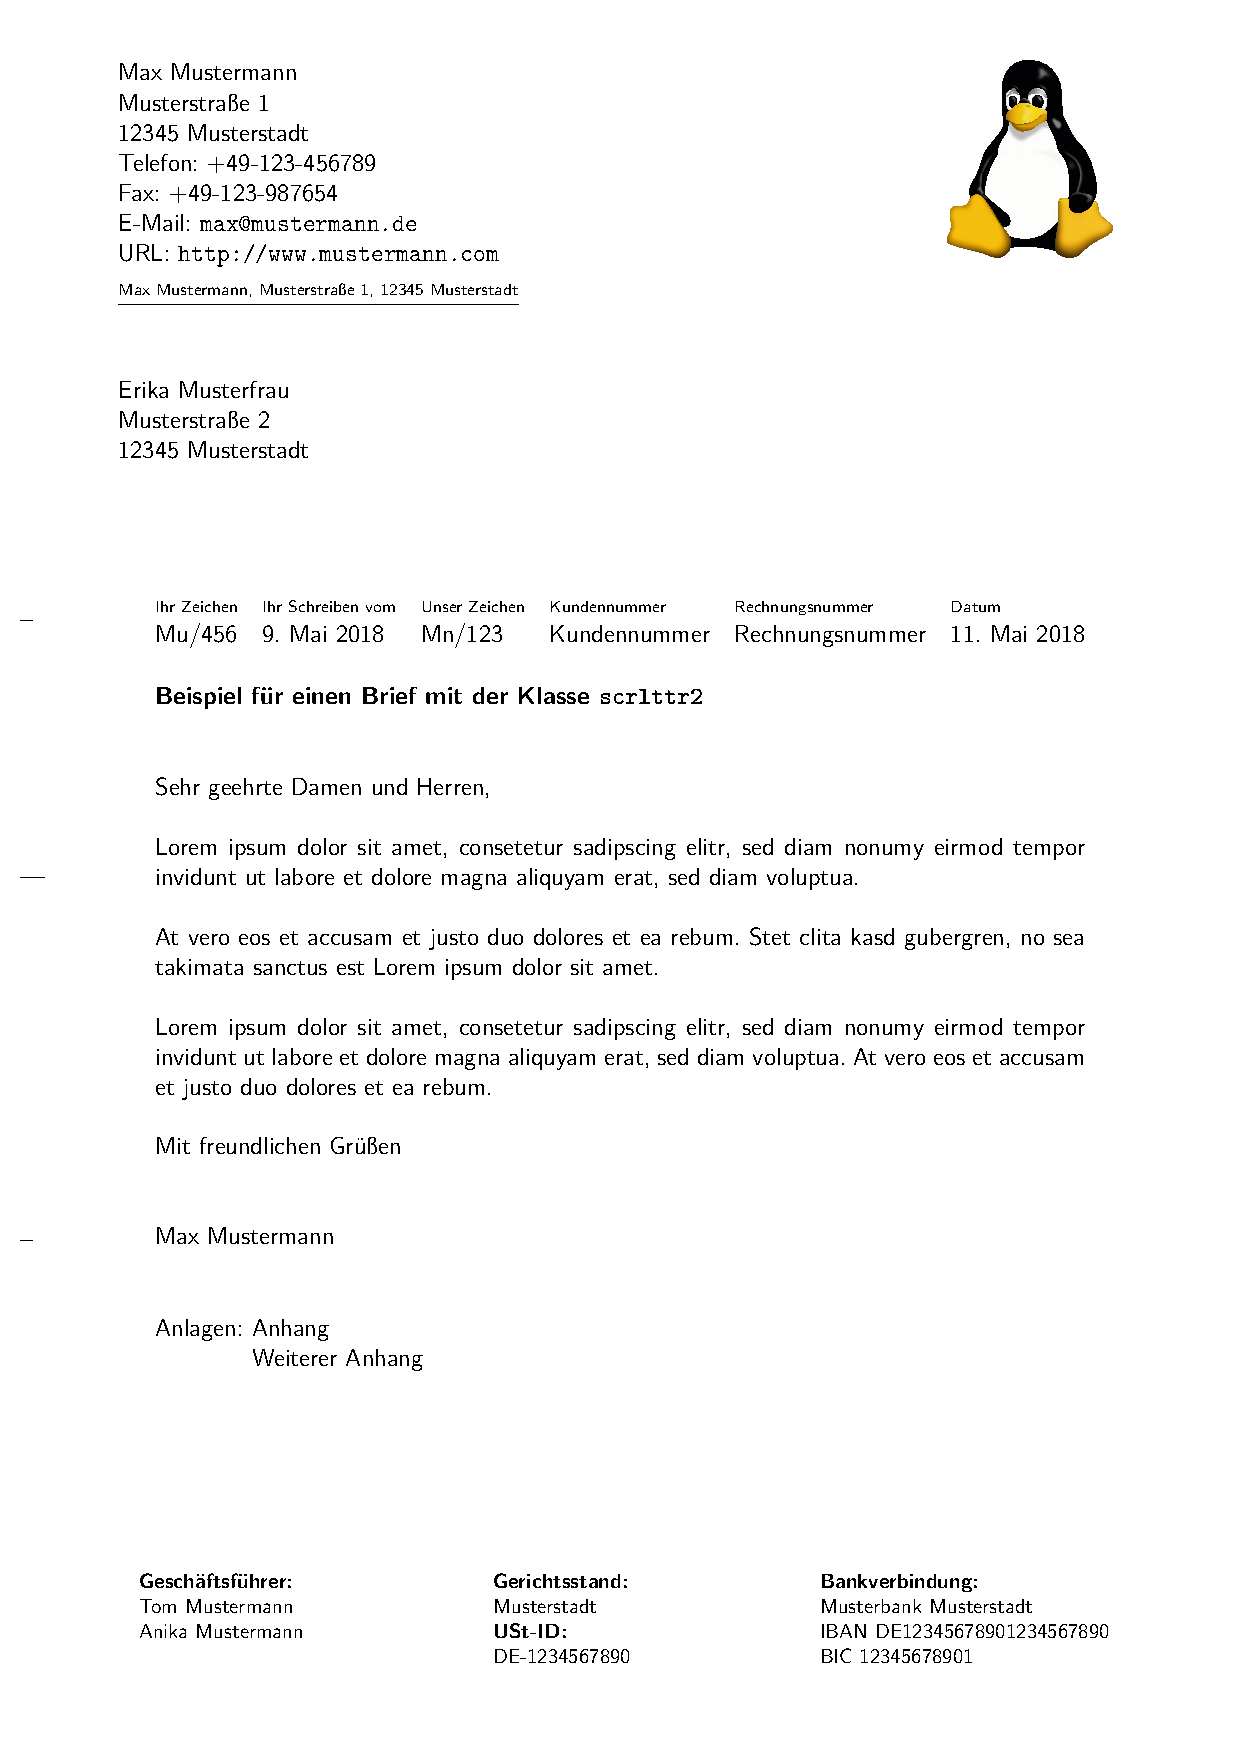
\includegraphics[page=1, width=.98\textwidth]{Beispiele/Brief_scrlttr2/brief_scrlttr2.pdf}}
    \caption{Resultat von Listing~\ref{beispielscrlttr2}}
    \label{fig_scrlttr2}
\end{figure}
